\documentclass[titlepage,a4paper]{article}
\usepackage{a4wide}
\usepackage[colorlinks=true,linkcolor=black,urlcolor=blue,bookmarksopen=true]{hyperref}
\usepackage{bookmark}
\usepackage{fancyhdr}
\usepackage[spanish]{babel}
\usepackage[utf8]{inputenc}
\usepackage[T1]{fontenc}
\usepackage{textcomp, gensymb}
\usepackage{graphicx}
\usepackage{float}
\usepackage{multicol}
\pagestyle{fancy} % Encabezado y pie de página
\fancyhf{}
\fancyhead[L]{TP1 - Grupo 1}
\fancyhead[R]{Análisis Numérico - FIUBA}
\renewcommand{\headrulewidth}{0.4pt}
\fancyfoot[C]{\thepage}
\renewcommand{\footrulewidth}{0.4pt}
\usepackage[utf8]{inputenc}

\begin{document}
\begin{titlepage} % Carátula
	%\hfill
\includegraphics[width=6cm]{logofiuba.jpg}
    \centering
    \vfill
    \Huge \textbf{Trabajo Práctico 1}
    \vskip2cm
    \Large [ 75.12 - 95.04 ] Análisis Numérico\\
    Curso 5 \\ 
    Primer cuatrimestre de 2020\\
    \vfill
    \begin{tabular}{ | l | l | } 
      \hline
        De Angelis Riva, Lukas & 103784 \\ \hline
        Gomez, Joaquín & 103735 \\ \hline
        Grassano, Bruno & 103855 \\ \hline
        Guillemi, Andrés & 104006\\ \hline 
        Rodriguez, Ezequiel & 103976 \\ \hline
        Romero, Adrián & 103371 \\ \hline
  	\end{tabular}
    \vfill
    \vfill
    \vfill
\end{titlepage}

\tableofcontents % Índice general

\newpage

\section{Introducción}\label{sec:intro}
En este trabajo práctico creamos un programa para la resolución de una ecuación diferencial de segundo orden con coeficientes constantes, que describe la posición y la velocidad de un péndulo, a través de los siguientes métodos numéricos aprendidos en la materia:
\begin{itemize}
    \item Runge Kutta de orden 1 (Euler)
    \item Runge Kutta de orden 4
\end{itemize}

Con este fin, creamos un script en Python que nos permite calcular las constantes necesarias para realizar las iteraciones de estos métodos. Luego procedimos a calcular y graficar los resultados obtenidos para posición, velocidad y energía en un intervalo de 20 segundos.

\section{Objetivos}\label{sec:objetivos}
El objetivo del trabajo es resolver una ecuación diferencial por medio de los métodos indicados anteriormente, para distintos pasos $h$ y comparar los órdenes de error. 

Además pretendemos estudiar el comportamiento de la energía $E$ para distintos tipos de amortiguamientos $b$.


\section{Análisis previo}
La siguiente es la ecuación diferencial que describe el ángulo de un péndulo simple $\theta$ en función del tiempo $t$ para las condiciones iniciales $\theta_0$ y $\theta'_0$:

\begin{center}
    EDO: \hspace{2mm} $\frac{d^2\theta}{dt^2}+\frac{b}{m}\frac{d\theta}{dt} +\frac{g}{l}\theta = 0$ \hspace{5mm} CI: \hspace{2mm} $\theta(0) = \theta_0$ \hspace{3mm} $\frac{d\theta}{dt}(0) = \theta'_0$
\end{center}

Dado que es una ecuación diferencial de segundo orden, para poder aplicar los métodos de RK1 y RK4, es necesario realizar un cambio de variables $u = \theta'$, resulta entonces:

\begin{center}
    EDOS: \hspace{2mm} $\theta' = u$ \hspace{15mm} CI: \hspace{2mm} $\theta(0) = \theta_0$ \\
    \hspace{15mm}$u' = -\frac{b}{m}u-\frac{g}{L}\theta$ \hspace{10mm} $u(0) = u_0$
\end{center}

Donde llamando $f(t, \theta, u) = -\frac{b}{m}u-\frac{g}{L}\theta$ podemos plantear los metodos de la siguiente manera:
    
Runge Kutta 1:

\begin{center}
    $u_{n+1} = u_{n} + h \cdot f(t_n, \theta_n, u_n)$\\
    $\theta_{n+1+} = \theta_{n} + h \cdot u_n$
\end{center}

Runge Kutta 4:

\begin{center}
    $u_{n+1} = u_{n} + \frac{h}{6} ( m_1 + 2m_2 + 2m_3 + m_4)$\\
    $\theta_{n+1+} = \theta_{n} + \frac{h}{6}  ( k_1 + 2k_2 + 2k_3 + k_4)$
\end{center}

Donde las constantes $k$ y $m$ cumplen:

\begin{multicols}{2}
\centering
$k_1 = u_n$\\
$k_2 = u_n + \frac{1}{2}hm_1$\\
$k_3 = u_n + \frac{1}{2}hm_2$\\
$k_4 = u_n + hm_3$\\
\columnbreak
$m_1 = f(t_n, \theta_n, u_n)$\\
$m_2 = f(t_n +\frac{1}{2}h, \theta_n+\frac{1}{2}hm_1, u_n+\frac{1}{2}hk_1)$ \\
$m_3 = f(t_n +\frac{1}{2}h, \theta_n+\frac{1}{2}hm_2, u_n+\frac{1}{2}hk_2)$ \\
$m_4 = f(t_n +h, \theta_n+hm_3, u_n+hk_3)$ \\
\end{multicols}

\newpage

\section{Resultados}

En las siguientes secciones mostraremos las soluciones aproximadas de la ecuación diferencial anterior, halladas por los método de Runge Kutta 1 y 4, y para distintos sets de parámetros: $b$, $m$, $L$, $\theta_0$, $\theta'_0$ y $h$.

Se muestran los primeros y los últimos cinco valores obtenidos para $\theta$ y $\theta'$.

\subsection{Caso 1: Sistema no amortiguado}

\begin{center}
    m = 1kg \hspace{3mm}
    L = 1m \hspace{3mm}
    b = 0 $Nsm^-1$ \hspace{3mm}
    h = 0.02s \hspace{3mm}
    $\theta_0$ = $30\degree$ \hspace{3mm}
    $\theta'_0 = 0\frac{\degree}{s}$ \hspace{3mm}
\end{center}

\begin{center}
    \begin{tabular}{| c | c | c | c | c | c|}
        \hline
       Tiempo[s] &\multicolumn{2}{|c|}{$\theta_n[rad]$} &\multicolumn{2}{|c|}{$\theta'[rad/s]$} \tabularnewline
        \hline
        &RK1&RK4&RK1&RK4\\
        \hline
        0.00&5.236e-01&5.236e-01&0.000e+00&0.000e+00\\
        0.02&5.236e-01&5.226e-01&-1.026e-01&-1.026e-01\\
        0.04&5.215e-01&5.195e-01&-2.053e-01&-2.047e-01\\
        0.06&5.174e-01&5.144e-01&-3.075e-01&-3.061e-01\\
        0.08&5.113e-01&5.073e-01&-4.089e-01&-4.062e-01\\
        ...&...&...&...&...\\
        19.92&3.125e+00&4.663e-01&6.048e+00&7.4058e-01\\
        19.94&3.246e+00&4.802e-01&5.435e+00&6.530e-01\\
        19.96&3.555e+00&4.924e-01&4.779e+00&5.577e-01\\
        19.98&3.451e+00&5.025e-01&4.142e+00&4.602e-01\\
        20.00&3.534e+00&5.100e-01&3.465e+00&3.600e-01\\
        \hline
    \end{tabular}
\end{center}

\subsection{Caso 2: Sistema amortiguado}

\begin{center}
    m = 1kg \hspace{3mm}
    L = 1m \hspace{3mm}
    b = 0.5 $Nsm^-1$ \hspace{3mm}
    h = 0.02s \hspace{3mm}
    $\theta_0$ = $30\degree$ \hspace{3mm}
    $\theta'_0 = 100\frac{\degree}{s}$ \hspace{3mm}
\end{center}

\begin{center}
    \begin{tabular}{| c | c | c | c | c | c|}
        \hline
       Tiempo[s] &\multicolumn{2}{|c|}{$\theta_n[rad]$} &\multicolumn{2}{|c|}{$\theta'[rad/s]$} \tabularnewline
        \hline
        &RK1&RK4&RK1&RK4\\
        \hline
        0.00&5.236e-01&5.236e-01&1.745e+00&1.745e+00\\
        0.02&5.585e-01&5.573e-01&1.625e+00&1.623e+00\\
        0.04&5.910e-01&5.885e-01&1.500e+00&1.495e+00\\
        0.06&6.210e-01&6.170e-01&1.369e+00&1.362e+00\\
        0.08&6.484e-01&6.429e-01&1.233e+00&1.226e+00\\
        ...&...&...&...&...\\
        19.92&1.041e-02&2.460e-04&1.123e-01&1.702e-02\\
        19.94&1.265e-02&5.841e-04&1.091e-01&1.677e-02\\
        19.96&1.483e-02&9.165e-04&1.055e-01&1.646e-02\\
        19.98&1.694e-02&1.242e-03&1.016e-01&1.609e-02\\
        20.00&1.897e-02&1.560e-03&9.722e-02&1.565e-02\\
        \hline
    \end{tabular}
\end{center}

\begin{figure}[H]
    \centering
    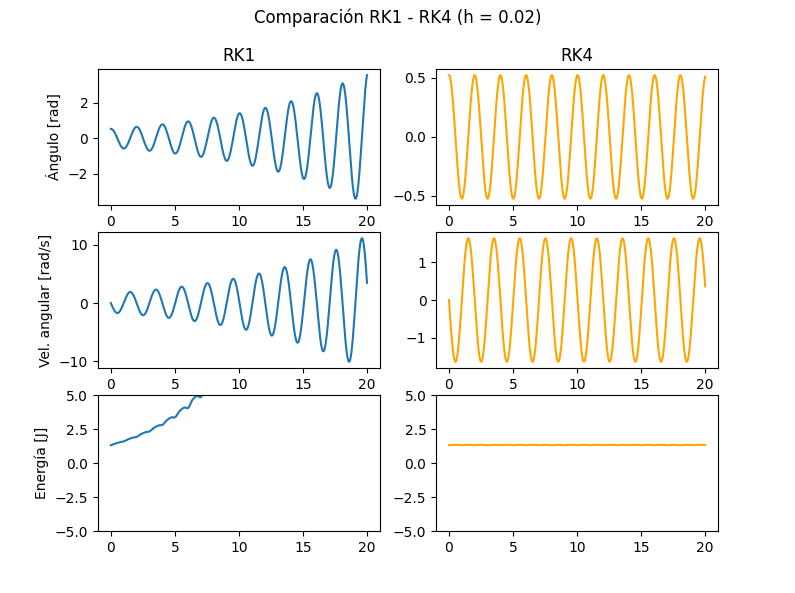
\includegraphics[scale = 0.4]{noAmortiguado1.png}
    \caption{}
\end{figure}

\begin{figure}[H]
    \centering
    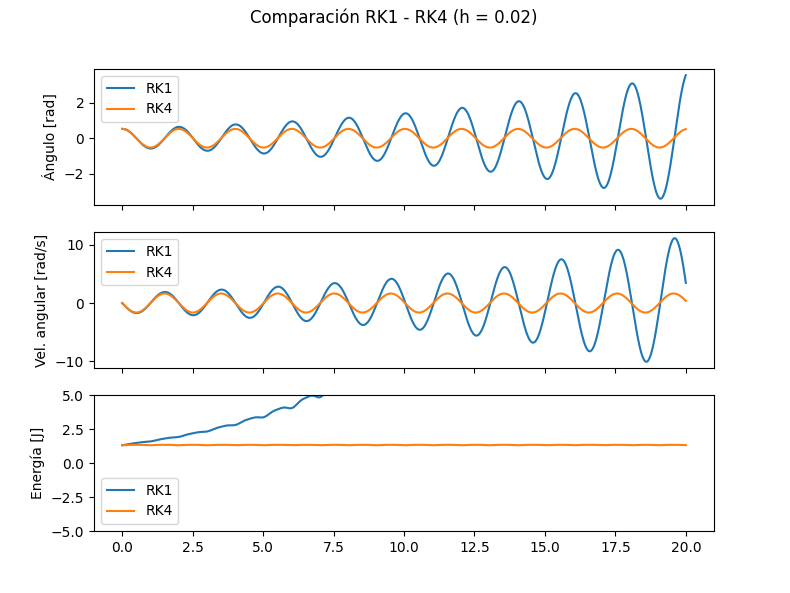
\includegraphics[scale = 0.4]{noAmortiguado2.png}
    \caption{}
\end{figure}

\begin{figure}[H]
    \centering
    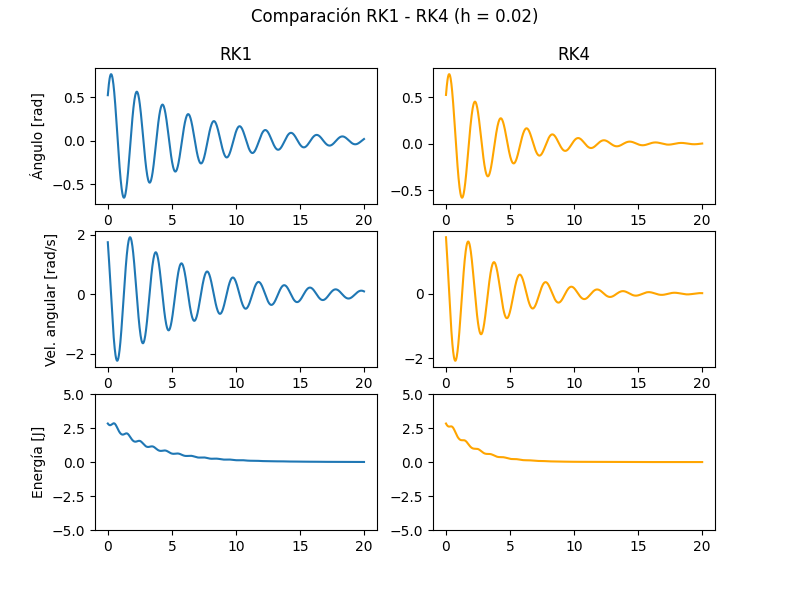
\includegraphics[scale = 0.4]{amortiguado1.png}
    \caption{}
\end{figure}

\begin{figure}[H]
    \centering
    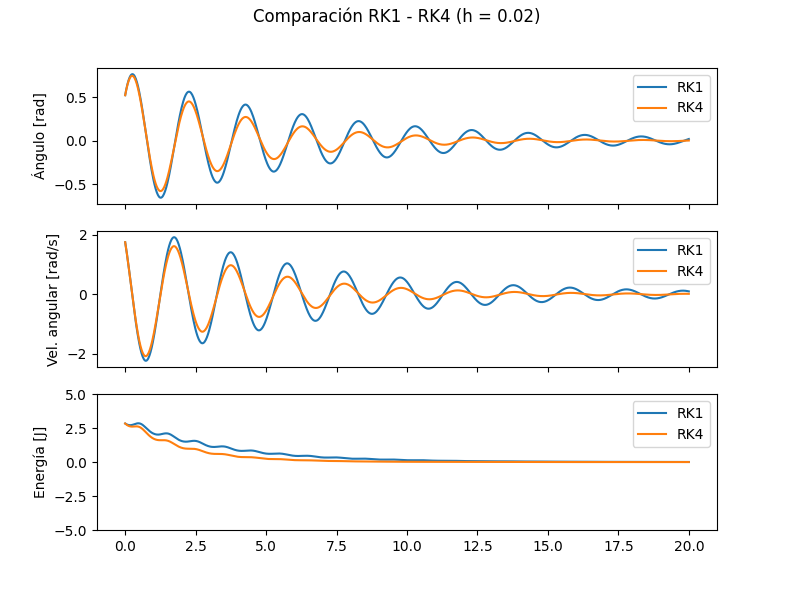
\includegraphics[scale = 0.4]{amortiguado2.png}
    \caption{}
\end{figure}

\section{Conclusiones}\label{sec:conclusiones}

    

    





\end{document}